\documentclass{article}
\usepackage[utf8x]{inputenc}
\usepackage[T1, T2A]{fontenc}
\usepackage[russian]{babel}
\usepackage{amsmath}
\usepackage{amssymb}
\usepackage{graphicx}
\setlength\parindent{0pt}
\usepackage[parfill]{parskip}
\pagenumbering{gobble}

\begin{document}
Вы попали в лабиринт, состоящий из нескольких комнат, соединенных системой двусторонних порталов. Каждый портал соединяет только одну пару комнат лабиринта. Порталом можно пользоваться неограниченное число раз. Вы появляетесь в комнате $v_1$ и прыжками перемещаетесь между комнатами. В комнате $v_6$ находится выход из лабиринта. Предположим, что каждый следующий портал для прыжка вы выбираете случайно и равновероятно среди всех порталов в этой комнате, включая портал до предыдущей комнаты. Найдите математическое ожидание количества прыжков до первого попадания в $v_6$.\\
Схема лабиринта:
\begin{figure}[h]
\center{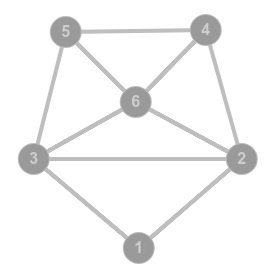
\includegraphics[width=0.3\textwidth]{maze}}
\end{figure}
\end{document}
